\AtBeginDocument{
  \catcode`_=12
  \begingroup\lccode`~=`_
  \lowercase{\endgroup\let~}\sb
  \mathcode`_="8000
}
\documentclass[times, zavrsni, numeric, utf8]{fer}
\usepackage{booktabs}
\usepackage{amsmath}
\usepackage{url}
\usepackage{algpseudocode}
\usepackage{graphicx}
\usepackage{subcaption}
\usepackage{float}
\usepackage{pdfpages}
\usepackage{adjustbox}
\usepackage{listings}
\usepackage{pifont}
\usepackage{pbox}
\usepackage{tikz}
\usepackage[unicode]{hyperref}
\usetikzlibrary{shapes.geometric, arrows, matrix, chains, positioning, decorations.pathreplacing}
\graphicspath{ {/home/jkneze/PycharmProjects/playing-card-recognition/} }
\newcommand{\source}[1]{\caption*{Izvor: {#1}} }
\newcommand{\code}[1]{\texttt{#1}}
\begin{document}

\tikzstyle{decision} = [diamond, minimum width=3cm, minimum height=1cm, text centered, draw=black, fill=blue!30]
\tikzstyle{process} = [rectangle, rounded corners, minimum width=3cm, minimum height=1cm,text centered, draw=black, fill=blue!30]
\tikzstyle{line} = [thick,->,>=stealth]
\tikzstyle{cloud} = [draw, ellipse, fill=red!20, minimum height=2em]

% TODO: Navedite broj rada.
\thesisnumber{4062}

% TODO: Navedite naslov rada.
\title{Sustav za raspoznavanje igraćih karata}

% TODO: Navedite vaše ime i prezime.
\author{Josip Knežević}

\maketitle

% Ispis stranice s napomenom o umetanju izvornika rada. Uklonite naredbu \izvornik ako želite izbaciti tu stranicu.
\includepdf[pages={1}]{izvornik.pdf}

% Dodavanje zahvale ili prazne stranice. Ako ne želite dodati zahvalu, naredbu ostavite radi prazne stranice.
\zahvala{}

\tableofcontents

\chapter{Uvod}
\label{chap:intro}
\hspace*{0.5cm}Računalni vid grana je umjetne inteligencije u području računarske znanosti, koja se bavi izgradnjom računarskih automata ili modela koji imaju sposobnost izvlačenja informacije iz slike. Razlog razvoja ovog područja je mogućnost računalne (elektroničke)vidne percepcije i digitalnog razumijevanja slike. Razumijevanje fotografija može biti viđeno kao odvajanje simboličke informacije iz slikovnih podataka koristeći modele napravljene uz pomoć geometrije, fizike, statistike i teorije učenja. Računalni vid također je opisan kao pothvat za automatizaciju i integraciju širokog spektra procesa i prezentaciju vizualne percepcije.\\
Područje primjene seže od industrijskih sustava za strojni vid, do istraživanja umjetne inteligencije i računala ili robota koji mogu shvatiti stvarni svijet oko njih. Neki primjeri primjene sustava računalnog vida su: \\
\hspace*{0.5cm}\textbullet{} Kontroliranje procesa \\
\hspace*{0.5cm}\textbullet{} Praćenje događaja (video nadzor, brojanje ljudi) \\
\hspace*{0.5cm}\textbullet{} Modeliranje objekata i okoline (analiza slika) \\
\hspace*{0.5cm}\textbullet{} Interakcija čovjeka i računala \\
\hspace*{0.5cm}Kao znanstvena disciplina, računalni vid se bavi teorijom iza umjetnih sustava koji dohvaćaju informacije iz slika. Slikovni podaci mogu poprimiti mnoge oblike, kao što su video sekvence, pogledi iz više kamera, ili više dimenzionalne podatke iz medicinskih skenera. \\
\hspace*{0.5cm}Kao tehnološka disciplina, računalni vid nastoji primijeniti svoju teoriju i modele za izgradnju sustava umjetnog vida.\\
\hspace*{0.5cm}Brojne kockarnice danas zainteresirane su za automatsko praćenje igara kako bi što lakše prikupile podatke relevantne za analizu igara. Budući da većina igara zahtjeva igranje standardnim poker kartama, pojavila se i potreba za uspješnim prepoznavanjem igraćih karata.
U ovom radu opisuje se postupak prepoznavanja jačine i oznake boje igraće karte na temelju morfoloških operacija te ostalih tehnika i algoritama obrade slike te računalnog vida.

\chapter{Obrada slike}
\label{chap:ip}
\section{Općenito o obradi slike}
\hspace*{0.5cm}Obrada slike (engl. \textit{image processing}) je bilo koja forma obrade informacije gdje je ulaz slika, npr. fotografija ili video sekvenca, dok je izlaz ili slika ili set karakterističnih parametara povezanih sa ulaznom slikom. Većina tehnika za obradu slike uključuju postupak gdje se slika smatra dvodimenzionalnim signalom. Pod obradom slike se danas većinom smatra obrada digitalne slike, ali optička i analogna obrada slike je također moguća. \\
\hspace*{0.5cm}Digitalna obrada slike podvrgavanje je numeričkih reprezentacija objekata seriji operacija s ciljem postizanja željenog rezultata. 
Proces obrade slike prolazi kroz tri glavna koraka: \\
\hspace*{0.5cm}\textbullet{} Učitavanje slike sa kamere ili direktno sa računala \\
\hspace*{0.5cm}\textbullet{} Manipulacija ili analiza slike \\
\hspace*{0.5cm}\textbullet{} Rezultat obrade slike (nova slika različita od originalne ili izvještaj o provedenoj analizi slike) \\
Tehnike obrade slike korištene u ovom radu opisane su u nastavku poglavlja.
\section{Matematička morfologija}
\label{schap:mm}
\hspace*{0.5cm}Matematička morfologija\cite{wikimm} je teorija i tehnika za analizu i obradu geometrijskih struktura, bazirana na teoriji skupova, teoriji rešetki, topologiji te slučajnim funkcijama. Zove se morfologija zato što morfološke operacije djeluju na oblik objekta. Najveća uporaba matematičke morfologije u praksi je upravo u obradi digitalnih slika. Operacije matematičke morfologije u početku su bile moguće samo na binarnim slikama, a kasnije je omogućena i nad slikama u tonovima sive boje (engl. \textit{grayscale}). Osnovni morfološki operatori su: \\
\hspace*{0.5cm}\textbullet{} Erozija (engl. \textit{erosion}) \\
\hspace*{0.5cm}\textbullet{} Dilatacija (engl. \textit{dilation}) \\
\hspace*{0.5cm}\textbullet{} Otvaranje (engl. \textit{opening}) \\
\hspace*{0.5cm}\textbullet{} Zatvaranje (engl. \textit{closing}) 

U ovom radu koriste se operacije binarne morfologije, koje su definirane pomoću teorije skupova. Slika je podskup euklidskog prostora $\mathbb{E}^{d}$ ili cjelobrojne rešetke $\mathbb{Z}^{d}$, gdje je $d$ dimenzija skupa.
\subsection{Strukturni element}
\hspace*{0.5cm}Osnovna ideja binarne morfologije je prolazak kroz sliku s jednostavnim, unaprijed određenim oblikom, koji kao rezultat pokaže koliko taj oblik (ne)pristaje obliku izvorne slike, ovisno o operaciji koju primjenjujemo. Taj predefinirani oblik naziva se strukturni element (engl. \textit{structure element}) koji je također binarna slika. Najčešće se označava slovom $B$. Najčešće korišteni strukturni elementi su: \\
\hspace*{0.5cm}\textbullet{} $E = \mathbb{R}^{2}$, $B$ je kružnica radijusa $r$, sa središtem u ishodištu \\
\hspace*{0.5cm}\textbullet{} $E = \mathbb{Z}^{2}$, $B$ je kvadrat dimenzija $3 \times 3$ sa središtem u ishodištu \\
\hspace*{0.5cm}\textbullet{} $E = \mathbb{Z}^{2}$, $B$ je "križ" sa središtem u ishodištu

\subsection{Erozija}
\hspace*{0.5cm}Erozija binarne slike $A$ strukturnim elementom $B$ definirana je kao: 
\begin{center}
\begin{equation}
A \ominus B = \{Y:y = inf[B(a)], a \in A\}
\end{equation}
\end{center}
gdje je $Y$ rezultat erodirane slike te je definiran kao \textit{infimum} (najmanja vrijednost) piksela $a$ ulazne slike $A$ na koju djeluje $B$.
Erozija skupa strukturnim elementom $B$ određenog oblika vrši izotropno smanjivanje (engl. \textit{thinning}) skupa. Važno je napomenuti da erozija nije komutativna, odnosno:
\begin{center}
\begin{equation}
A \ominus B \neq B \ominus A
\end{equation}
\end{center}

\subsection{Dilatacija}
\hspace*{0.5cm}Dilatacija binarne slike $A$ strukturnim elementom $B$ definirana je kao:
\begin{center}
\begin{equation}
A \oplus B = \{Y:y = sup[B(a)], a \in A\}
\end{equation}
\end{center}
gdje je $Y$ rezultat dilatirane slike te je definiran kao \textit{supremum} (najveća vrijednost) piksela $a$ ulazne slike $A$ na koju djeluje $B$.
Dilatacija je komplementarna eroziji, prema tome ima suprotan učinak od erozije, odnosno, dilatacija skupa strukturnim elementom $B$ određenog oblika vrši izotropno debljanje (ekspanziju) skupa. Za razliku od erozije, dilatacija je komutativna:
\begin{center}
\begin{equation}
A \oplus B = B \oplus A
\end{equation}
\end{center}
Dilatacija ima i svojstvo asocijativnosti:
\begin{center}
\begin{equation}
(A \oplus B) \oplus C = A \oplus (B \oplus C)
\end{equation}
\end{center}

\subsection{Otvaranje}
\hspace*{0.5cm}Otvaranje je kombinacija prethodno opisanih morfoloških operatora. Prvo se izvršava erozija između $A$ i $B$ te se na rezultat erozije izvršava dilatacija s $B$. Formalno se zapisuje kao:
\begin{center}
\begin{equation}
A \circ B = (A \ominus B) \oplus B
\end{equation}
\end{center}
Otvaranje skupa strukturnim elementom $B$ kružnog oblika može se interpretirati kao kotrljanje kruga unutar oblika (engl. \textit{rolling ball algorithm}) 
\subsection{Zatvaranje}
\hspace*{0.5cm}Zatvaranje je također, kao i otvaranje, kombinacija erozije i dilatacije, ali s obrnutim redoslijedom operatora. Prvo se vrši dilatacija strukturnim elementom $B$ te nakon toga erozija. Formalno se zapisuje kao:
\begin{center}
\begin{equation}
A \bullet B = (A \oplus B) \ominus B
\end{equation}
\end{center}
Zatvaranje skupa strukturnim elementom $B$ kružnog oblika može se interpretirati kao kotrljanje kruga s vanjske strane oblika.
\subsection{Pogodi i promaši transformacija}
\label{schap:hom}
\hspace*{0.5cm}Pogodi i promaši transformacija (engl. \textit{Hit-and-miss transform}) koristi se za traženje određene strukture u slici. Definirana je kao:
\begin{center}
\begin{equation}
A \otimes (J, K) = (A \ominus J) \cap (A^{c} \ominus K)
\end{equation}
\end{center}
gdje je $A^{c}$ komplement skupa $A$, a $J$ i $K$ su strukturni elementi koji zadovoljavaju uvjet:
\begin{center}
\begin{equation}
J \cap K = \emptyset
\end{equation}
\end{center}
Ova relacija govori sljedeće: ukoliko je neki piksel $x$ ulazne slike $A$ "pogođen" strukturnim elementom $J$ (odnosno odgovara traženom obliku) i istovremeno je promašen strukturnim elementom $K$ (odnosno odgovara pozadini ulazne slike $A$), onda je $x$ ispravan i stavljamo ga na izlaz.

\section{Izlučivanje značajki slike}
\label{schap:extract}
\hspace*{0.5cm}Za uspješno prepoznavanje igraćih karata potrebno je prethodno izvršiti niz operacija koje omogućuju izdvajanje karte od ostalih objekata koji se nalaze na slici. Prilikom toga koriste se brojni poznati algoritmi i tehnike računalnog vida poput detekcije rubova, pronalaženja kontura te perspektivne transformacije. 
\subsection{Detekcija rubova}
\label{schap:edgedetect}
\hspace*{0.5cm}Detekcija rubova jedan je od fundamentalnih problema koji se javljaju pri računalnoj obradi slike. Rubovi su definirani kao nagle promjene u intenzitetu susjednih piksela i predstavljaju granice objekata na slici, odnosno koriste se za detekciju položaja ili orijentacije tih objekata. Danas se najčešće koristi Cannyev detektor rubova\cite{canny1986comp}. Cannyev algoritam možemo razmatrati kao filtar koji ulaznu crno-bijelu sliku obrađuje na način da na izlaznoj slici postoje samo rubovi ili ne-rubovi. Cannyev detektor rubova je koristan kod povećanja kontrasta te smanjenja šuma na slici. Upravo zbog toga pomaže pri izolaciji karte sa slike. Da bi Cannyev detektor rubova uspješno obavio posao, potrebno je napraviti sljedeće korake: 
\begin{enumerate}
\item Primijeniti Gaussov filtar\cite{wikigauss} 
\item Pronaći gradijente intenziteta slike 
\item Usporedba s pragom (engl. \textit{threshold}) 
\item Stanjivanje rubova 
\end{enumerate}

Gaussov filtar koristi se kako bi se smanjili detalji u slici, a djeluje na sliku tako da, u odnosu na izvornu, izgleda zamagljeno. Veličina Gaussova filtra se predaje Cannyevom detektoru kao parametar. \\
Gradijent je vektor koji pokazuje smjer najveće promjene intenziteta. Računa se vodoravna i okomita komponenta gradijenta. Ukupni intenzitet računa se kao:
\begin{center}
\begin{equation}
G = \sqrt{G_x^{2} + G_y^{2}}
\end{equation}
\end{center} 
Smjer gradijenta računa se prema formuli:
\begin{center}
\begin{equation}
\theta = \arctan(\frac{G_y}{G_x})
\end{equation}
\end{center}
pri čemu se dobiveni kut zaokružuje na $0^{\circ}$, $45^{\circ}$, $90^{\circ}$ i $135^{\circ}$. \\
Cannyev detektor koristi dva praga, gornji (engl. \textit{high}) i donji (engl. \textit{low}) prag. Pikseli intenziteta većeg od gornjeg praga prihvaćaju se kao rubovi, dok se pikseli intenziteta nižeg od donjeg praga odbacuju. Ostali pikseli, koji se nalaze između dva praga dodatno se pokušavaju izolirati, pomoću 8 susjednih piksela. Oni pikseli koji u svom 8-susjedstvu imaju barem jedan piksel koji je iznad gornjeg praga se prihvaćaju kao rubovi.\\
Pri postupku stanjivanja rubova, uklanjaju se sve neželjene točke, koje bi mogle uzrokovati lažno prepoznati rub. Konačni rezultat je stanjivanje rubova na debljinu od samo jednog piksela, što povećava mogućnost točnog detektiranja traženog objekta na slici. \\
Rezultat primjene Cannyeva detektora rubova kroz korake može se vidjeti na slici \ref{fig:canny}
\begin{figure}[H]
\begin{subfigure}{.5\textwidth}
  \centering
  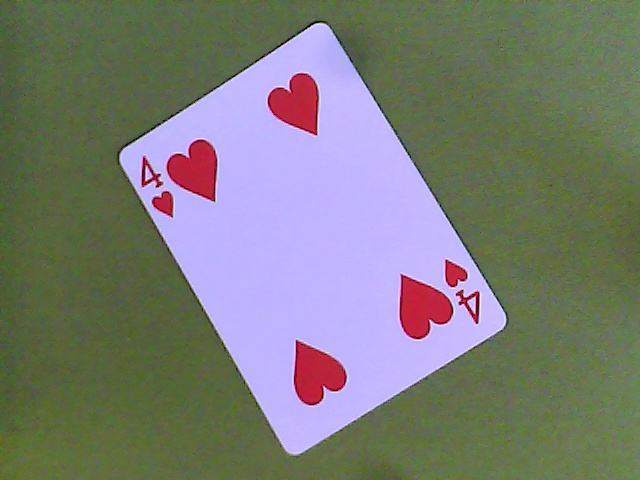
\includegraphics[width=.8\linewidth]{sve-karte/img13.jpg}
  \caption{Izvorna slika}
  \label{fig:orig4herc}
\end{subfigure}%
\begin{subfigure}{.5\textwidth}
  \centering
  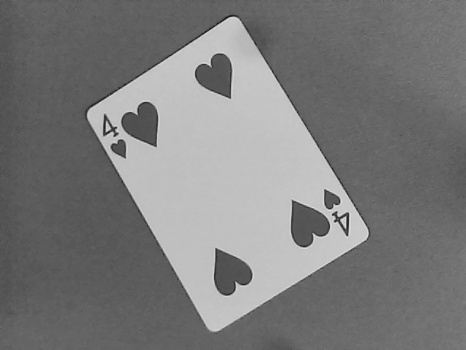
\includegraphics[width=.8\linewidth]{grayscale.jpg}
  \caption{Slika sivih tonova}
  \label{fig:gray}
\end{subfigure}
\begin{subfigure}{.5\textwidth}
  \centering
  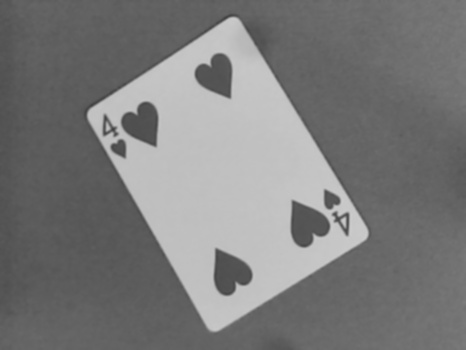
\includegraphics[width=.8\linewidth]{blurred.jpg}
  \caption{Primjena Gaussova filtra}
  \label{fig:gaussblur}
\end{subfigure}%
\begin{subfigure}{.5\textwidth}
  \centering
  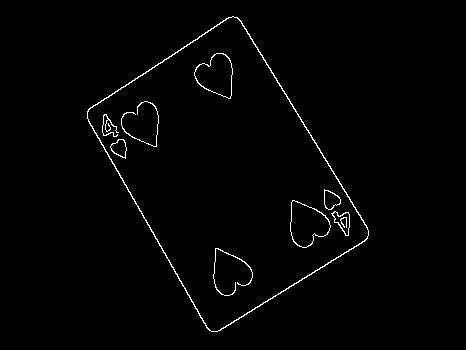
\includegraphics[width=.8\linewidth]{edged.jpg}
  \caption{Istaknuti rubovi}
  \label{fig:edged}
\end{subfigure}
\caption{Proces detekcije rubova}
\label{fig:canny}
\end{figure}

\subsection{Pronalaženje kontura}
\label{schap:contours}
\hspace*{0.5cm}U računalnom vidu, konture opisuju granice nekog oblika u slici. Koriste se za mnoge zadatke računalnog vida poput praćenja objekata, prepoznavanja oblika, segmentacije, itd. Konture su zapravo nizovi točaka koji predstavljaju neku vrstu krivulje na slici. Iako na prvi pogled konture stvaraju isti efekt kao postupak opisan u \ref{schap:edgedetect}, zadaća pronalaska kontura je ipak složenija. Prilikom pronalaženja rubova, oni se također stavljaju u odabranu vrstu hijerarhije. Zbog toga možemo dohvatiti samo vanjske konture ukoliko to želimo. U Suzukijevom\cite{suzukicontours} radu dan je efikasan algoritam za pronalazak kontura koji se koristi s manjim modifikacijama i u \code{OpenCV}-u\cite{opencv}.

\subsection{Perspektivna transformacija}
\label{schap:persp}
\hspace*{0.5cm}Perspektivna transformacija usko je povezana uz pojam perspektivne projekcije. Perspektivna projekcija je model koji je bliži čovjeku. U praksi je često zanimljiva vrsta projekcije kod koje projekcijske zrake nisu paralelne, kao kod ljudskog vida ili fotografije. Fotografija predstavlja projekciju scene iz trodimenzionalnog prostora na dvodimenzionalnu ravninu. Projekcijske zrake u tom slučaju izviru iz jedne točke na konačnoj udaljenosti od projekcijske ravnine. Općeniti slučaj perspektivne projekcije pokazan je na slici \ref{fig:perspective}
\begin{figure}[H]
  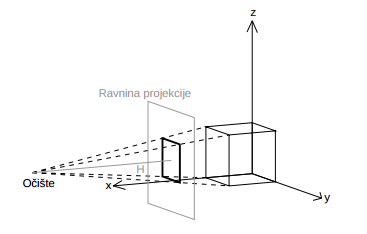
\includegraphics{perspective.png}
  \caption{Općeniti slučaj perspektivne projekcije}
  \label{fig:perspective}
  \source{Interaktivna računalna grafika kroz primjere u \textit{OpenGL}-u\cite{cupicmihajlovic} }
\end{figure}

Perspektivna transformacija\cite{oreillycv} spaja dvije zasebne slike koje su alternativne projekcije istog trodimenzionalnog objekta projicirane na dvije zasebne ravnine. Jednostavan primjer se dobiva kada se očište nalazi u ishodištu koordinatnog sustava, a gledište na $z$ osi (slika \ref{fig:exampleperspective}). Očište i vrhovi lika spojeni su spojnicama koje probadaju ravninu projekcije $z = H$. Na $x$ i $y$-koordinatnim osima označene su koordinate vrhova i probodišta ravnine projekcije.
\begin{figure}[H]
\centering
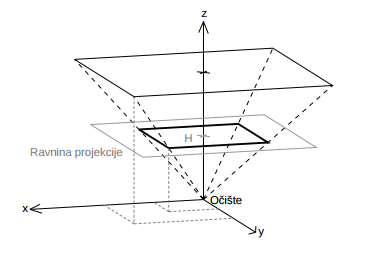
\includegraphics{xospp.png}
\caption{Perspektivna projekcija}
\label{fig:exampleperspective}
\source{Interaktivna računalna grafika kroz primjere u \textit{OpenGL}-u\cite{cupicmihajlovic}}
\end{figure}
Analizu za $x$-os radimo prema slici \ref{fig:perpanaliza}. Iz slike vidimo da postoje slični trokuti $0 - H - T_P$ i $0 - T_z - T$. Za $x$-os vrijedi sljedeće:
\begin{equation}
\frac{T_{P,x}}{H} = \frac{T_x}{T_z} \Rightarrow T_{P, x} = {T_x}\cdot\frac{H}{T_z}
\end{equation}
Analogno, za $y$-os vrijedi:
\begin{equation}
\frac{T_{P,y}}{H} = \frac{T_y}{T_z} \Rightarrow T_{P, y} = {T_y}\cdot\frac{H}{T_z}
\end{equation}
\begin{figure}[H]
\centering
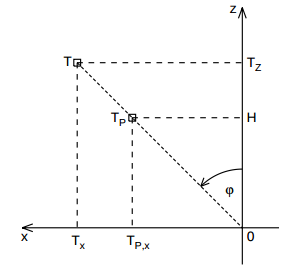
\includegraphics{xos2dpp.png}
\caption{Perspektivna projekcija}
\label{fig:perpanaliza}
\source{Interaktivna računalna grafika kroz primjere u \textit{OpenGL}-u\cite{cupicmihajlovic}}
\end{figure}
Ukoliko sve točke zapišemo pomoću homogene koordinate, matrica perspektivne projekcije može se zapisati kao:
\begin{equation}
				P =
				\begin{bmatrix}
					1 & 0 & 0 & 0\\
					0 & 1 & 0 & 0\\
					0 & 0 & 0 & \frac{1}{H}\\
					0 & 0 & 0 & 0
				\end{bmatrix}
\end{equation}
\\
$z$-koordinata točke koja se dobije perspektivnom projekcijom preko prethodno izvedene matrice iznosi 0 zbog toga što točka leži u ravnini projekcije. \\
Perspektivna transformacija ključan je postupak u pretprocesiranju slike prije pozivanja glavnog dijela programa. Ukoliko nije dobro izvršena, prepoznavanje karte neće uspjeti jer karta neće biti pravilno dignuta u ptičju perspektivu te će time biti onemogućeno daljnje procesiranje karte.

\chapter{Razmatrani pristupi za raspoznavanje karata}
\label{chap:methods}
\hspace*{0.5cm}Tijekom početnog istraživanja problema, u obzir su se uzele tri metode za prepoznavanje jačine i oznake boje karte:
\begin{enumerate}
\item Optičko prepoznavanje znakova (engl. \textit{Optical character recognition, OCR}) u kombinaciji sa detektorom za oznake boje
\item Neuronska mreža
\item Tehnike obrade slike
\end{enumerate}

\section{OCR i detektor oznaka boje}
\hspace*{0.5cm}Budući da je prepoznavanje znakova uspješno rješeno i dobro dokumentirano, ovo je bio prilično logičan prvi korak ka ostvarenju sustava za prepoznavanje igraćih karata. Budući da se sva informacija potrebna za prepoznavanje jačine karte nalazi u kutovima, OCR bi lagano pronašao koja je jačina karte, ukoliko se dobro izoliraju kutovi. OCR ne može razriješiti znakove koji predstavljaju oznaku boje (herc, tref, pik, karo) karte, pa je trebalo naći drugi način kako je odrediti. Za to bi bio pogodan detektor objekata, odnosno četiri detektora kojima bi prepoznavali o kojoj oznaci boje se radi. Sam proces treniranja detektora ne bi bio problem, ali ideja nije realizirana zbog mogućeg velikog broja lažnih pozitiva (engl. \textit{false positives}). Naime, često bi mogao zamijeniti same oznake boje (npr. herc i pik), ali također bi mogao za nešto što uopće nije oznaka boje reći da je pronašao traženu oznaku. 

\section{Neuronska mreža}
\hspace*{0.5cm}Druga ideja je bilo učenje neuronskim mrežama. Na ulaz neuronske mreže bi se stavila karta, a izlaz bi bio vektor koji bi pokazivao koji smo tip karte dobili. Budući da se raspolaže ograničenim skupom na ulazu i izlazu, neuronska mreža bi davala jako dobre rezultate. Dovoljna bi bila neuronska mreža koja bi raspoznavala je li karta brojčana ($2 - 10$) ili je označena slovom ($A, J, Q, K$). Na ulaz bi se stavile $52$ karte u raznim uvjetima, a izlaz bi bio dvodimenzionalni vektor koji bi rekao je li karta brojčana ili je označena slovom. Nakon toga bi se išlo u daljnje procesiranje, odnosno gledali bi je li karta crna ili crvena te nakon toga uzeti najvjerojatniju opciju između četiri oznake boje. Nakon što je naučena, neuronska mreža bi lako prepoznala kartu koja bi joj došla na ulaz. Glavni nedostatak neuronske mreže je taj što bi trebalo prikupiti mnoštvo primjeraka za učenje.\\
Iako bi neuronska mreža dala jako dobre rezultate, od realizacije se odustalo zbog nedovoljnog poznavanja neuronskih mreža. 


\section{Tehnike obrade slike}
\hspace*{0.5cm}Metoda odabrana za realizaciju temelji se na tehnikama obrade slike koje su opisane u poglavlju \ref{chap:ip}. Tijek izvođenja prikazan je na slici \ref{fig:flowchart}. Realizacija se djelomično temelji na radu \cite{martinspoker}. U svakom koraku izvođenja koristi se niz funkcija koje vode ka točnom prepoznavanju karte. \\
U prvom koraku učitava se izvorna slika u bilo kojem formatu podržanom u \code{OpenCV}-u. Nakon toga sa slike se izolira karta što se postiže 
pronalaženjem kontura. Kako bi se smanjila vjerojatnost pogrešnog klasificiranja karte, napravljen je postupak u kojem se odlučuje je li izoliranom dijelu slike prevladava crvena ili crna boja. \\
Sljedeći korak je raspoznavanje tipa karte, odnosno je li karta označena brojem ili slovom te izolacija kuteva u kojima je sadržana informacija bitna za daljnju klasifikaciju. Ukoliko je karta brojčana onda ulazimo u funkciju za detektiranje broja karte, inače ulazimo u funkciju u kojoj detektiramo slovo. Izlaz iz bilo koje od prethodne dvije funkcije je ulaz za detekciju oznake boje (herc, tref, pik, karo). \\
Više o samoj implementaciji sustava napisano je u poglavlju \ref{chap:impl}. 
\begin{figure}[H]
	\centering
	\begin{tikzpicture}[node distance = 2.5cm, auto]
		% Place nodes
		\node [process] (imgget) {Izvorna slika};
		\node [process, below of=imgget] (cardfind) {Izolacija karte};
		\node [process, below of=cardfind] (colourdet) {Crvena ili crna karta};
		\node [process, below of=colourdet] (typedet) {Detektiraj tip karte};
		\node [process, below of=typedet] (symfind) {Izolacija simbola};
		\node [decision, below of=symfind] (ispic) {Broj / Slovo};
		\node [process, right of=ispic, xshift=+2cm] (numdet) {Detektiraj broj};
		\node [process, left of=ispic, xshift=-2cm] (rankdet) {Detektiraj slovo};
		% Enhanced by colour detection
		\node [process, below of=ispic] (symdet) {Detektiraj oznaku boje};


		% Draw edges
		\draw [line] (imgget) -- (cardfind);
		\draw [line] (cardfind) -- (colourdet);
		\draw [line] (colourdet) -- (typedet);
		\draw [line] (typedet) -- (symfind);
		\draw [line] (symfind) -- (ispic);
		\draw [line] (ispic) -- node {broj} (numdet);
		\draw [line] (ispic) -- node {slovo} (rankdet);
		\draw [line] (rankdet) -- (symdet);
		\draw [line] (numdet) -- (symdet);
	\end{tikzpicture}
	\caption{Tijek izvođenja programa}
	\label{fig:flowchart}
\end{figure}


\chapter{Implementacija}
\label{chap:impl}
\hspace*{0.5cm}Za realizaciju zadanog zadatka odabran je programski jezik \code{Python} uz pomoć biblioteka \code{OpenCV} te \code{numpy}. Iako se većinom barata \code{OpenCV} funkcijama te bi dio koda vezan uz njih bio gotovo identičan kao i u jeziku \code{C++}, \code{Python} je odabran zbog jednostavnosti u realizaciji dijelova programske potpore koji nisu usko vezani uz \code{OpenCV} funkcije. 
\section{Izvorna slika}
\hspace*{0.5cm}Postupak učitavanja izvorne slike jedan je od osnovnih postupaka za početak bilo koje aplikacije iz područja računalnog vida i obrade slike. 
Izvorna slika može biti u bilo kojem obliku podržanom u \code{OpenCV}-u (\textit{bitmap, portable image formats, JPEG, TIFF datoteke}). Za učitavanje slike koristi se ugrađena \code{OpenCV} funkcija
\begin{center}
\code{cv2.imread(filename[, flags]) $\rightarrow$ retval}.
\end{center}
\code{filename} se predaje preko komandne linije prilikom pokretanja programa. Ukoliko je uspješno učitana slika, šalje se na daljnju obradu, inače se izlazi iz programa. 
\section{Izolacija karte}
\label{schap:cardiso}
\hspace*{0.5cm}Nakon što smo učitali sliku, potrebno je naći kartu na slici te provesti nekoliko koraka pretprocesiranja slike koristeći tehnike obrade slike navedene u poglavlju \ref{schap:extract}. \\
Nakon provedenog postupka detekcije rubova (\ref{schap:edgedetect}) potrebno je pronaći najveću četverokutnu konturu na slici. Glavni dio posla odrađuje funkcija prototipa:
\begin{center}
\code{cv2.findContours(image, mode, method[, contours[, hierarchy[, offset]]]) $\rightarrow$ contours, hierarchy}
\end{center}
kojoj se preko argumenta \code{image} predaje slika na kojoj želimo pronaći konture. Slika mora biti jednokanalna, odnosno slika sivih tonova ili binarizirana slika. Drugi važan argument funkcije jest \code{mode}, preko kojega se određuje koje konture će biti tražene. Budući da se traži najveća četverokutna kontura, treba se koristiti način \code{RETR_LIST} koji sprema sve konture bez hijerarhije u listu. Zbog uštede memorije, preko argumenta \code{method} predaje se \code{CHAIN_APPROX_SIMPLE} koji umjesto svih točaka kontura, uzima samo njihove krajnje točke. U slučaju četverokuta to bi bila 4 vrha četverokuta. Rezultat se može vidjeti na slici \ref{fig:conts}.
\begin{figure}[H]
\centering
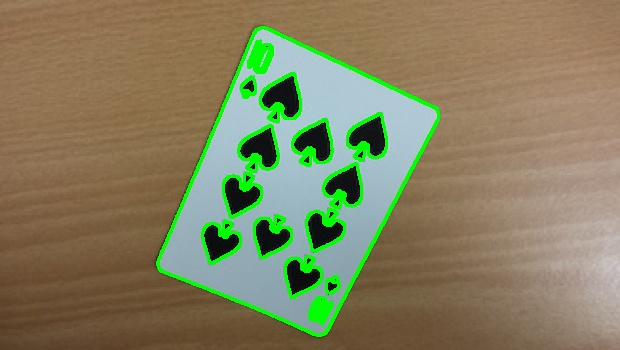
\includegraphics[width=.8\linewidth]{sve_konture.jpg}
\caption{Pronađene konture prikazane na izvornoj slici}
\label{fig:conts}
\end{figure}

Sada je potrebno od svih označenih kontura uzeti samo onu koja je četverokutna i najveća. Konture se aproksimiraju ugrađenom funkcijom \code{cv2.approxPolyDP} koja aproksimira krivulju poligona s određenom preciznošću. Ukoliko dođemo do konture koja je aproksimirana s četiri točke, zaključujemo da smo našli kartu i tu konturu uzimamo kao relevantnu, a ostale odbacujemo (slika \ref{fig:onecont}). Nakon toga radimo perspektivnu transformaciju opisanu u poglavlju \ref{schap:persp} kako bi mogli sliku slati na daljnju obradu. Perspektivna transformacija nam omogućuje ispravno prepoznavanje karte jer stavlja kartu u uspravan položaj bez ikakvog nagiba (slika \ref{fig:warppersp}). Matricu perspektivne transformacije dobijemo korištenjem funkcije prototipa:
\begin{center}
\code{cv2.getPerspectiveTransform(src, dst) $\rightarrow$ retval},
\end{center}
gdje su parametrom \code{src} zadane koordinate četiri vrha iz izvorne slike, a parametrom \code{dst} koordinate ta četiri vrha u izlaznoj slici. Sama transformacija vrši funkcijom 
\begin{center}
\code{cv2.warpPerspective(src, M, dsize)}, 
\end{center}
gdje je argument \code{dsize}, koji predstavlja širinu i visinu nove slike, postavljen na $250 \times 350$ što zadovoljava omjer standardne karte ($5 : 7$).

\begin{figure}[H]
\begin{subfigure}{.5\textwidth}
  \centering
  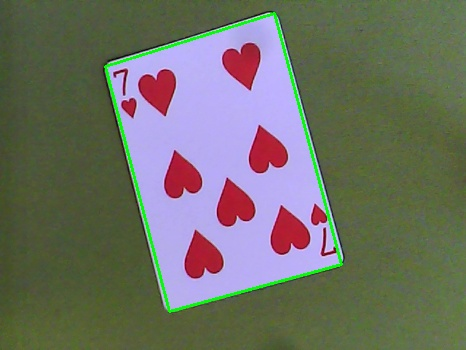
\includegraphics[width=1.0\linewidth]{outline.jpg}
  \caption{Pronađena karta na izvornoj slici}
  \label{fig:onecont}
\end{subfigure}%
\begin{subfigure}{.5\textwidth}
  \centering
  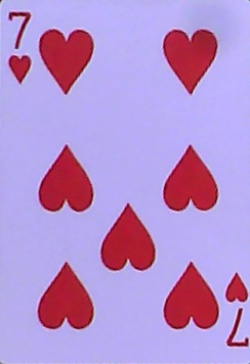
\includegraphics[width=.5\linewidth]{warped.jpg}
  \caption{Karta nakon perspektivne transformacije}
  \label{fig:warppersp}
\end{subfigure}
\caption{Detektiranje karte i prilagodba za daljnju obradu}
\label{fig:carddet}
\end{figure} 

\section{Određivanje tipa karte}
\label{schap:typcoldet}
\subsection{Obojenje karte}
\label{schap:colordet}
\hspace*{0.5cm}Korak koji povećava vjerojatnost ispravnog klasificiranja igraćih karata jest podjela karti na crne i crvene. Osim što će smanjiti prostor pretraživanja, ovaj korak će spriječiti lažnu klasifikaciju karte. Naime, ako se pogleda oznaka za herc i pik, možemo vidjeti da su one vrlo slične (slika \ref{fig:hercpik}) pa bi pogodi i promaši transformacija (opisana u poglavlju \ref{schap:hom}) mogla krivo klasificirati kartu. Ukoliko ispravno provedemo raspoznavanje crvenih i crnih karti ovo se neće dogoditi, jer su uz crvene karte vezani herc i karo, a uz crne pik i tref. 
\begin{figure}[H]
\begin{subfigure}{.5\textwidth}
  \centering
  
\includegraphics[width=.2\linewidth]{simboli/spade_flipped.png}
  \caption{Rotirani binarizirani znak pik}
  \label{fig:sf}
\end{subfigure}%
\begin{subfigure}{.5\textwidth}
  \centering
  
\includegraphics[width=.2\linewidth]{simboli/heart.png}
  \caption{Binarizirani znak herc}
  \label{fig:herc}
\end{subfigure}
\caption{Prikaz sličnosti između pojedinih oznaka boje}
\label{fig:hercpik}
\end{figure} 

Kao ulaz funkciji za određivanje obojenja karte predaje se karta oblika kao na slici \ref{fig:warppersp}. Prvi korak je pretvoriti sve bijele piksele na karti u crne (slika \ref{fig:blackb}). Razlog ovome je taj što crni piksel ima vrijednosti \code{(0, 0, 0)} te će nakon ovog koraka svi pikseli različiti od te vrijednosti biti najvećim dijelom crveni, što olakšava određivanje obojenja karte. 
\begin{figure}[H]
\centering
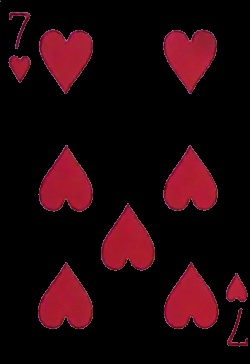
\includegraphics[width=.5\linewidth]{blackb.jpg}
\caption{Crna pozadina}
\label{fig:blackb}
\end{figure}
Sljedeći zadatak kojim se dokazuje većinsko prisustvo crvene boje je micanje svih plavih i zelenih komponenti boje sa slike prikazane na \ref{fig:blackb}. Ovime se postiže efekt isticanja crvene boje, ukoliko je ona prisutna na slici. Budući da je pozadina potpuno crna (vrijednosti pozadinskih piksela su \code{(0, 0, 0)}), svaki piksel koji nije potpuno crn se jednostavno zamijeni sa vrijednošću \code{(0, 0, val)} (slika \ref{fig:redness}), gdje je \code{val} vrijednost crvene komponente piksela na toj poziciji na slici. \\
\hspace*{0.5cm}Nakon što je napravljeno isticanje crvene komponente na slici, lagano se provjeri je li karta ima crno ili crveno obojenje. Dovoljno je pregledati gornji lijevi kut karte te ukoliko se pokaže da postoji dovoljan broj crvenih piksela onda karta ima crveno obojenje, inače je crno. Za svaki piksel iz gornjeg lijevog kuta provjeravamo koja je komponenta dominantna. Ukoliko je najveći dio površine gornjeg lijevog kuta crven, karta se uzima kao crvena. Površina koju zauzima gornji lijevi kut dobivena je empirijski. Početna točka gornjeg lijevog kuta je $(5, 5)$, a visinom se proteže do $30\%$ ukupne visine karte te širinom do $15\%$ ukupne širine karte.
\begin{figure}[H]
\begin{subfigure}{.5\textwidth}
  \centering
  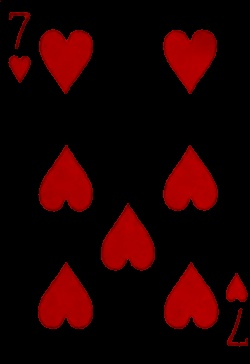
\includegraphics[width=.778\linewidth]{crvena.jpg}
  \caption{Crvena karta nakon isticanja crvene komponente}
  \label{fig:crv}
\end{subfigure}%
\begin{subfigure}{.5\textwidth}
  \centering
  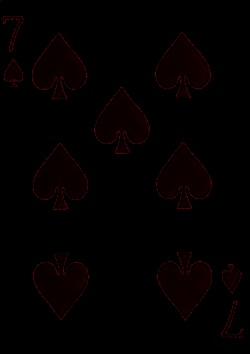
\includegraphics[width=.8\linewidth]{crna.jpg}
  \caption{Crna karta nakon isticanja crvene komponente}
  \label{fig:crn}
\end{subfigure}
\caption{Isticanje crvene komponente na kartama s crnom pozadinom}
\label{fig:redness}
\end{figure} 

\subsection{Detektiranje tipa karte}
\label{schap:typedet}
\hspace*{0.5cm}Detektiranje tipa karte je postupak koji također kao i postupak otkrivanja obojenja karte (\ref{schap:colordet}) smanjuje prostor pretraživanja. Naime, karta se šalje dalje na obradu ovisno kojeg je tipa. Ukoliko je karta označena brojem, onda se pokušava otkriti koji je broj vezan za nju ($2 - 10$), a ako je označena znakom onda se pokušava otkriti koji je znak vezan za nju ($J, Q$ ili $K$). Poseban slučaj je detektiranje karte označene slovom $A$, koja se također šalje na brojčanu analizu zbog načina na koji se detektiraju jačine brojčanih karata (detaljnije opisano u poglavlju \ref{schap:detval}). \\
Postupak detektiranja tipa karte se svodi, kao i u poglavlju \ref{schap:cardiso}, na pronalaženje četverokutne konture unutar slike. Razlika je u tome što je sad na ulazu slika iz "ptičje" perspektive (slika \ref{fig:warppersp}), a ne izvorna slika. Ovaj postupak je dobar, jer sve karte koje su označene znakom (izuzetak već spomenuta karta $A$) imaju kvadrat unutar karte. Ako se uspije detektirati takav kvadrat (slika \ref{fig:queenconts}, onda se može sa sigurnošću reći da je ta karta označena znakom ($J, Q$ ili $K$). Za razliku od postupka navedenog u poglavlju \ref{schap:cardiso}, ovdje se dodaje još jedno ograničenje. Osim što se aproksimira kvadrat ($4$ vrha), uvodi se i ograničenje na površinu konture. Budući da postupak traženja kontura pronalazi sve konture na slici, ograničenjem površine se osigurava da će se pronaći tražena kontura pomoću koje će se razlikovati karte označene brojem i karte označene znakom. Empirijski je utvrđeno postavljanje granice na $40000$, odnosno, odbacit će se sve konture čija je površina manja od $40000$ piksela. 
\begin{figure}[H]
\centering
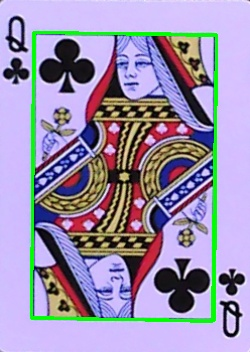
\includegraphics[width=.5\linewidth]{qcont.jpg}
\caption{Određivanje tipa karte, kvadrat unutar karte}
\label{fig:queenconts}
\end{figure}
\section{Izolacija simbola}
\label{schap:symiso}
\hspace*{0.5cm}Izolacija simbola vrši se zbog ubrzanja programa. Budući da se sva potrebna informacija nalazi u kutovima karte, dovoljno je pronaći te izolirati kutove u nove matrice. Temelj ove izolacije je \textit{Floodfill} algoritam.
\subsection{\textit{Floodfill} algoritam}
\label{schap:floodfill}
\hspace*{0.5cm}\textit{Floodfill} algoritam jedan je od poznatih algoritama koji se koristi za popunjavanje dijela slike odabranom bojom. Koristi tri parametra: \code{cvor}, \code{trazena_boja}, \code{zamjenska_boja}. Njegov zadatak je pretražiti sve čvorove u listi ili polju koji su povezani s početnim čvorom i obojani traženom bojom, te ih obojiti u zamjensku boju. Pretraživanje se vrši u $4$ smjera: istok, zapad, sjever, jug ili u $8$ smjerova: istok, zapad, sjever, jug, sjeveroistok, sjeverozapad, jugoistok, jugozapad. \textit{Floodfill} je zapravo verzija pretraživanja u dubinu (engl. \textit{Depth First Search, DFS}). Unutar \code{OpenCV} biblioteke postoji već ugrađena funkcija za algoritam \textit{Floodfill} koja je korištena u ovom radu. % TODO: stavi algoritam 

\subsection{Izolacija uporabom \textit{Floodfill} algoritma}
\label{schap:ffiso}
\hspace*{0.5cm}Na ulazu se raspolaže crno-bijelom binarnom slikom (bijela pozadina, crn ostatak slike). Prostor pretraživanja je gornji lijevi kut slike koji sadrži simbole. Algoritam pronalaženja simbola u slici je sljedeći:
\begin{enumerate}
  \item Za svaki piksel u gornjem lijevom kutu slike:
  \begin{enumerate}
    \item Ako je piksel crni, algoritmom \textit{Floodfill} popuni nakupinu piksela (engl. \textit{blob}) bijelom bojom. (efekt brisanja)
    \item Načini \code{XOR} slike sa izbrisanom nakupinom piksela te binarnom slikom s ulaza
  \end{enumerate}
  \item Ukoliko su pronađene dvije nakupine piksela na izlaznim slikama nakon operacije \code{XOR}, postavi prvu nakupinu kao jačinu, a drugu kao oznaku boje.
\end{enumerate}

Nakon \code{XOR} funkcije pronalazi se minimalni pravokutnik koji opisuje pronađenu nakupinu piksela te se time olakšava označavanje simbola jačine i oznake boje na originalnoj karti. Detaljni prikaz je na slici \ref{fig:blobs}.

\begin{figure}[H]
\begin{subfigure}{.5\textwidth}
  \centering
  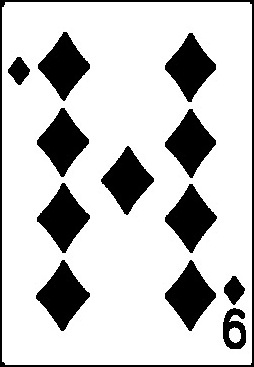
\includegraphics[width=.8\linewidth]{nflooded0.jpg}
  \caption{Izbrisan simbol $9$}
  \label{fig:fl90}
\end{subfigure}%
\begin{subfigure}{.5\textwidth}
  \centering
  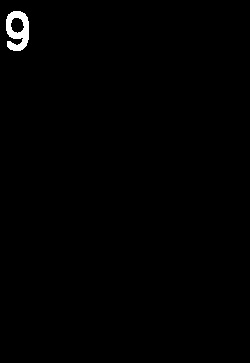
\includegraphics[width=.8\linewidth]{xor.jpg}
  \caption{Slika nakon \code{XOR}-a}
  \label{fig:xor90}
\end{subfigure}
\begin{subfigure}{.5\textwidth}
  \centering
  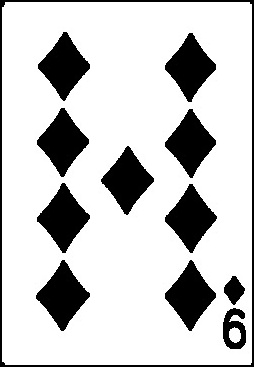
\includegraphics[width=.8\linewidth]{nflooded1.jpg}
  \caption{Izbrisan simbol karo}
  \label{fig:fl91}
\end{subfigure}%
\begin{subfigure}{.5\textwidth}
  \centering
  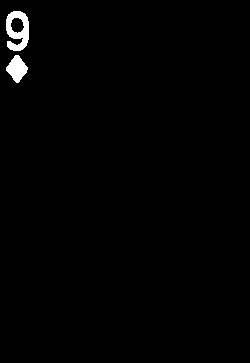
\includegraphics[width=.8\linewidth]{xor1.jpg}
  \caption{Konačna slika nakon \code{XOR}-a}
  \label{fig:xor91}
\end{subfigure}
\begin{subfigure}{.5\textwidth}
  \centering
  
\includegraphics[width=.2\linewidth]{rank.jpg}
  \caption{Izolirana jačina karte}
  \label{fig:rank}
\end{subfigure}%
\begin{subfigure}{.5\textwidth}
  \centering
  
\includegraphics[width=.2\linewidth]{suit.jpg}
  \caption{Izolirana oznaka boje karte}
  \label{fig:suit}
\end{subfigure}
\caption{Izolacija simbola}
\label{fig:blobs}
\end{figure}

\section{Detekcija brojčane vrijednosti}
\label{schap:detval}
\hspace*{0.5cm}Brojčane karte su karte $2 - 10$. Specifičnost tih karti je da u središnjem dijelu imaju upravo onoliko nakupina piksela kolika je jačina te karte. Prema toma, određivanje vrijednosti brojčane karte radit će se jednostavno preko brojanja nakupina piksela u središtu karte.\\
Kako bi to bilo moguće, potrebno je binarizirati ulaznu sliku te izbrisati kutove iz slike (slika \ref{fig:bindel}).
\begin{figure}[H]
\begin{subfigure}{.5\textwidth}
  \centering
  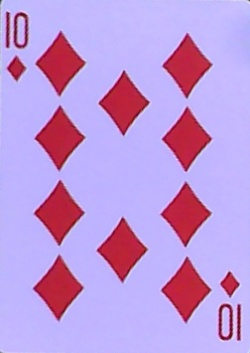
\includegraphics[width=.8\linewidth]{blobcount.jpg}
  \caption{}
  \label{fig:blcnt}
\end{subfigure}%
\begin{subfigure}{.5\textwidth}
  \centering
  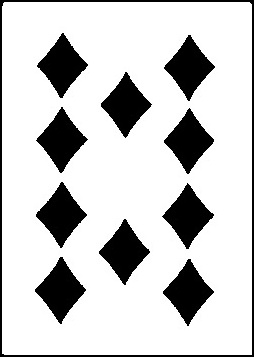
\includegraphics[width=.8\linewidth]{nbezkuteva.jpg}
  \caption{}
  \label{fig:binary}
\end{subfigure}
\caption{Binarizacija i brisanje kuteva}
\label{fig:bindel}
\end{figure}

Budući da se radi sa slikom nad kojom su prethodno izvršene brojne transformacije, postoji mogućnost da u nekom od znakova u središtu karte postoji prekid u nakupini piksela, što bi rezultiralo dvostrukim brojanjem tog znaka, što remeti mogućnost ispravnog klasificiranja karte. Da bi se spriječio takav slučaj, koriste se operacije matematičke morfologije opisane u poglavlju \ref{schap:mm}. U ovom slučaju koristi se dilatacija i otvaranje kako bi dobili nakupine piksela koje nemaju nikakve prekide (slika \ref{fig:dilandopen}). Funkcija za prebrojavanje je jednostavna. Koristeći \textit{floodfill} algoritam prebriše se jedan po jedan blob i sa svakim brisanjem se povećava brojač. Konačna vrijednost brojača je i vrijednost karte.
\begin{figure}[H]
\centering
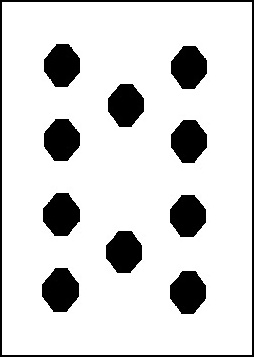
\includegraphics[width=.5\linewidth]{nclosed.jpg}
\caption{Binarizirana slika nakon primjene operacija dilatacije i otvaranja}
\label{fig:dilandopen}
\end{figure}

\section{Detekcija vrijednosti karti s oznakom slova} % TODO: koji vrag s ovim nazivom, nisam pametan
\label{schap:detroyal}
\hspace*{0.5cm}Za razliku od brojčanih karti, karte čija je vrijednost slovo (osim $A$) nemaju nikakvu povezanost između broja nakupina piksela u sredini i jačine. Za određivanje jačine koristi se pogodi i promaši transformacija opisana u poglavlju \ref{schap:hom}, s prilagodbom na zadani problem. Za ovaj korak je važna ispravna izolacija simbola (\ref{schap:ffiso}) jer se izolirani simboli jačine koriste za usporedbu s unaprijed napravljenim strukturnim elementima oznaka boje (slika \ref{fig:patterns}). Prije obavljanja poklapanja s predloškom (engl. \textit{template matching}) izolirani simbol jačine karte i strukturni element skalirani su na iste veličine. Izolirani simbol za trenutnu kartu se uspoređuje sa sva tri strukturna elementa, a karti se pridružuje ona jačina za koju je pogodi i promaši transformacija dala najveći postotak poklapanja. 
\begin{figure}[H]
				\centering
				\begin{subfigure}[b]{0.14\textwidth}
					\centering
					
\includegraphics[width=\textwidth]{templates-rank/image23.png}
					\caption{}
				\end{subfigure}
				\begin{subfigure}[b]{0.14\textwidth}
					\centering
					
\includegraphics[width=\textwidth]{templates-rank/image25.png}
					\caption{}
				\end{subfigure}
				\begin{subfigure}[b]{0.15\textwidth}
					\centering
					
\includegraphics[width=\textwidth]{templates-rank/image24.png}
					\caption{}
				\end{subfigure}
				\caption{Strukturni elementi (jačina)}
				\label{fig:patterns}
			\end{figure}

Iako postoji u biblioteci \code{scipy}, za pogodi i promaši transformaciju napravila se posebna funkcija, koja je u suštini radila poklapanje s predloškom, odnosno, nakon što su skalirani izolirani simbol i strukturni element, za svaki piksel unutar izoliranog simbola se gledao isti taj piksel unutar strukturnog elementa, te ukoliko je pogođen, povećao bi se brojač, te bi se na kraju uzeo postotak pogođenih piksela za određeni simbol i strukturni element (slika \ref{fig:homprobs}). Funkcija se izvršavala u zadovoljavajućem vremenu zbog korištenja visoko-optimirane biblioteke \code{numpy}, ali i zbog relativno malih veličina slika koje se uspoređuju. 
\begin{figure}[H]
\begin{subfigure}{.5\textwidth}
  \centering
  
\includegraphics[width=0.18\linewidth]{rankjack.jpg}
  \caption{Izolirani simbol}
  \label{fig:rjack}
\end{subfigure}%
\begin{subfigure}{.5\textwidth}
  \centering
  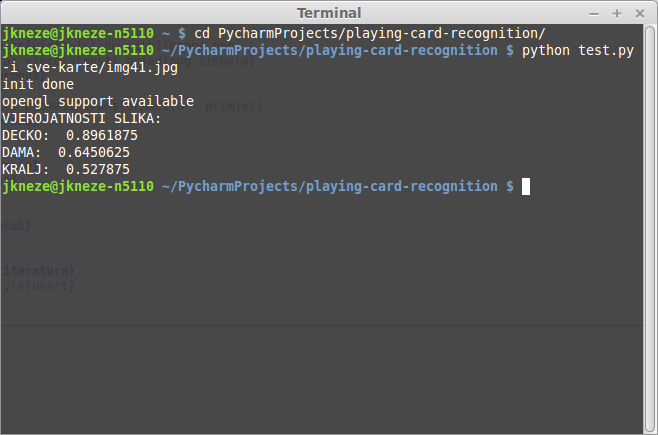
\includegraphics[width=1\linewidth]{probs.png}
  \caption{Prikaz vjerojatnosti pojedinog simbola}
  \label{fig:termout}
\end{subfigure}
\caption{Pogodi i promaši transformacija (jačina) - primjer}
\label{fig:homprobs}
\end{figure}
\section{Detekcija oznake boje}
\label{schap:suitdet}
\hspace*{0.5cm}Detekcija oznake boje se, kao i prethodno opisane karte sa slovima, vrši pomoću prilagođene pogodi i promaši transformacije pomoću unaprijed definiranih strukturnih elemenata prikazanih na slici \ref{fig:suitse}. U ovom koraku koristi se obojenje karte (poglavlje \ref{schap:colordet}) pri čemu se smanjuje prostor pretraživanja i mogućnost pogrešnog klasificiranja svodi na minimum. Nakon toga, izolirana oznaka boje (\ref{schap:ffiso}) te strukturni elementi se skaliraju na istu veličinu, te se nakon toga vrši pogodi i promaši transformacija potpuno isto kao i u poglavlju \ref{schap:detroyal} samo sa različitim izoliranim simbolom i različitim strukturnim elementima.

\begin{figure}[H]
				\centering
				\begin{subfigure}[b]{0.14\textwidth}
					\centering
					
\includegraphics[width=\textwidth]{templates-rank/image29.png}
					\caption{}
				\end{subfigure}
				\begin{subfigure}[b]{0.14\textwidth}
					\centering
					
\includegraphics[width=\textwidth]{templates-rank/image28.png}
					\caption{}
				\end{subfigure}
				\begin{subfigure}[b]{0.15\textwidth}
					\centering
					
\includegraphics[width=\textwidth]{templates-rank/image31.png}
					\caption{}
				\end{subfigure}
				\begin{subfigure}[b]{0.15\textwidth}
					\centering
					
\includegraphics[width=\textwidth]{templates-rank/image30.png}
					\caption{}
				\end{subfigure}
				\caption{Strukturni elementi (oznaka boje)}
				\label{fig:suitse}
			\end{figure}
Primjer klasifikacije može se vidjeti na slici \ref{fig:homsuits}. 
\begin{figure}[H]
\begin{subfigure}{.5\textwidth}
  \centering
  
\includegraphics[width=0.18\linewidth]{suitsym.jpg}
  \caption{Izolirani simbol}
  \label{fig:suitsymbol}
\end{subfigure}%
\begin{subfigure}{.5\textwidth}
  \centering
  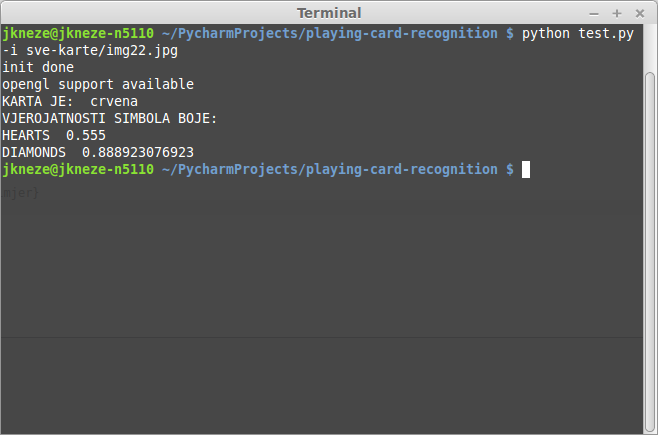
\includegraphics[width=1\linewidth]{probssuit.png}
  \caption{Prikaz vjerojatnosti pojedinog simbola}
  \label{fig:termout1}
\end{subfigure}
\caption{Pogodi i promaši transformacija (oznaka boje) - primjer}
\label{fig:homsuits}
\end{figure}
\section{Grafički izlaz programa}
\hspace*{0.5cm}Nakon provedenih svih koraka, grafički izlaz programa nam daje pregled svih bitnih informacija na jednoj slici (obojenje, jačina, oznaka boje). Također, na temelju informacije iz poglavlja \ref{schap:ffiso} označuju se pravokutnici oko simbola jačine i oznake boje kao dokaz da su pronađeni i ispravno izolirani iz cijele karte (slika \ref{fig:recognition}). Za prikaz informacije koristi se nova slika na kojoj su napisani osnovni podaci o originalnoj slici (slika \ref{fig:info}). Osim osnovnih podataka, prikazan je i podatak o vremenu izvođenja cijelog programa, od učitavanja izvorne slike pa sve do detekcije oznake boje, koja je zadnji korak. 
\begin{figure}[H]
\begin{subfigure}{.5\textwidth}
  \centering
  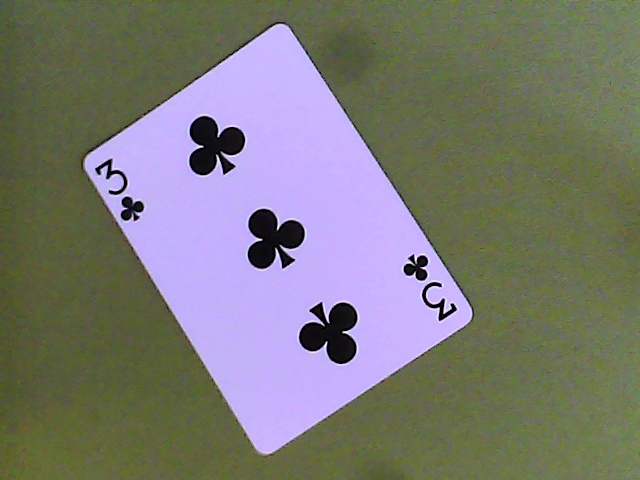
\includegraphics[width=0.8\linewidth]{sve-karte/img11.jpg}
  \caption{Izvorna slika}
  \label{fig:sourceimg}
\end{subfigure}%
\begin{subfigure}{.5\textwidth}
  \centering
  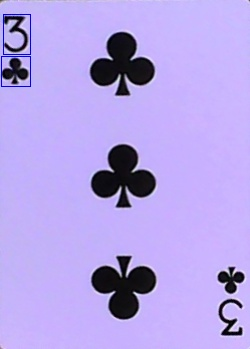
\includegraphics[width=0.5\linewidth]{recognition.jpg}
  \caption{Pronađeni i ispravno izolirani simboli}
  \label{fig:recognition}
\end{subfigure}
\begin{center}
\begin{subfigure}{.5\textwidth}
  \centering
  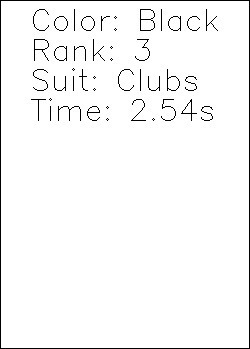
\includegraphics[width=0.5\linewidth]{newinfo.jpg}
  \caption{Informacije o izvornoj slici}
  \label{fig:info}
\end{subfigure}
\end{center}
\caption{Grafički izlaz programa}
\label{fig:guioutput}
\end{figure}


\chapter{Testiranje}
\label{chap:test}
\hspace*{0.5cm}Demonstracija rada sustava prikazana je kroz prijašnja poglavlja, a ovdje se koncetrira na sveukupnu efikasnost sustava. U jednom snopu ima $52$ karte, $13$ jačina, svaka u $4$ oznake boje. Svaka karta je slikana s malom rotacijom, na svijetlo zelenoj pozadini s dobrim osvjetljenjem (slika \ref{fig:testimages}). U ovakvim uvjetima sustav se pokazao kao dovoljno dobar i raspoznaje $51$ od $52$ karte u snopu. Jedina karta koju nije uspio prepoznati bila je $A$ pik, koji je problem zbog svog specifičnog izgleda. Sa slike \ref{fig:aceproblem} vidi se zašto se krivo prepoznaje ova karta. Naime, nakon primjene morfoloških operacija dilatacije i otvaranja nad kartom, u sredini su ostale dvije nakupine piksela, što je algoritmu za prepoznavanje brojeva značilo broj 2, te je stoga ova karta krivo klasificirana. Problem bi se mogao izbjeći s korištenjem drugog strukturnog elementa, ali to bi se vjerojatno negativno odrazilo na ostatak karti iz snopa, pa bi ukupna efikasnost sustava bila manja. Drugi način kojim se može riješiti ovaj problem jest klasificiranje $A$ karti putem pogodi i promaši transformacije, što bi vrlo vjerojatno rezultiralo točnom klasifikacijom znaka $A$. \\
Važno je reći da sustav ispravno prepoznaje u svakoj od 52 testne karte oznaku boje, iako se po rezultatima vjerojatnosti oznaka boje može reći da kod crvenih simbola, karo dominira nad hercom, a kod crnih pik nad trefom, odnosno, ukoliko je na ulazu znak karo, dominantno će se prepoznati da je to karo (s razlikom u prosjeku većom od $0.3$), dok za slučaj kada je na ulazu herc, onda je razlika u nekim slučajevima minimalna, ali ipak se ispravno prepozna herc. Slična situacija je i sa crnim kartama. U tablici \ref{table:stats} se vide rezultati testiranja nad testnim kartama sa slike \ref{fig:testimages}, kao i vrijeme potrebno za detekciju pojedine karte. 
Iz tablice {\ref{table:stats}} se vidi da je vrijeme potrebno za obradu jedne slike od početka do kraja otprilike jednako za sve karte, što se i očekivalo. Možda se na prvu čini kako bi opisanim postupkom prepoznavanja karti više vremena trebalo u prosjeku za detekciju karti označenih slovom, to nije slučaj, jer se prema dijagramu \ref{fig:flowchart} vidi da se podjednak broj koraka radi u oba slučaja, a funkcije u kojima se otkriva broj, odnosno slovo su slične složenosti. 

\begin{figure}[H]
		\centering
		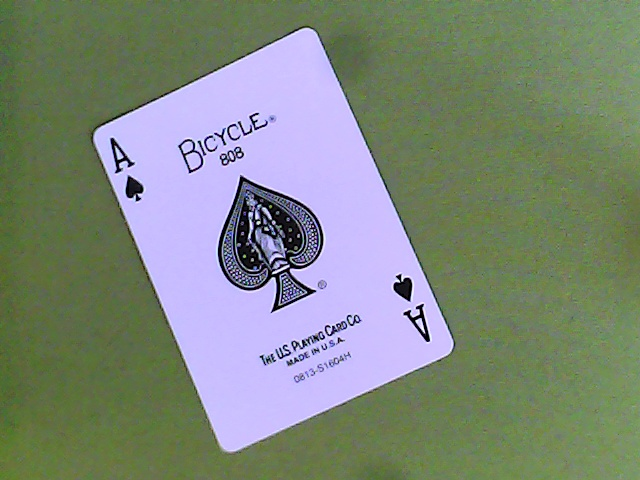
\includegraphics[width=0.06\linewidth]{sve-karte/img0}
		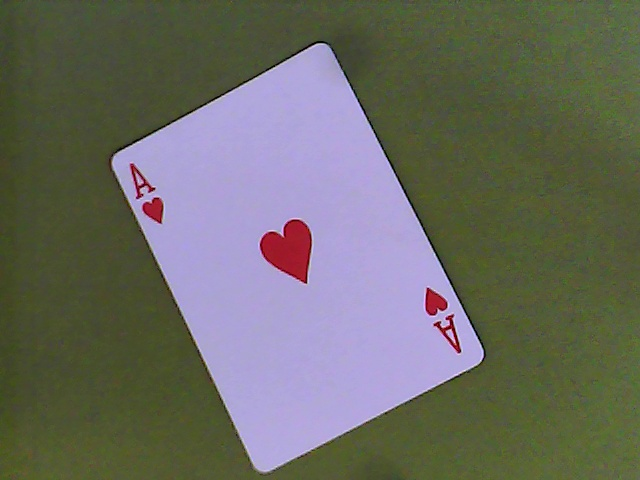
\includegraphics[width=0.06\linewidth]{sve-karte/img1}
		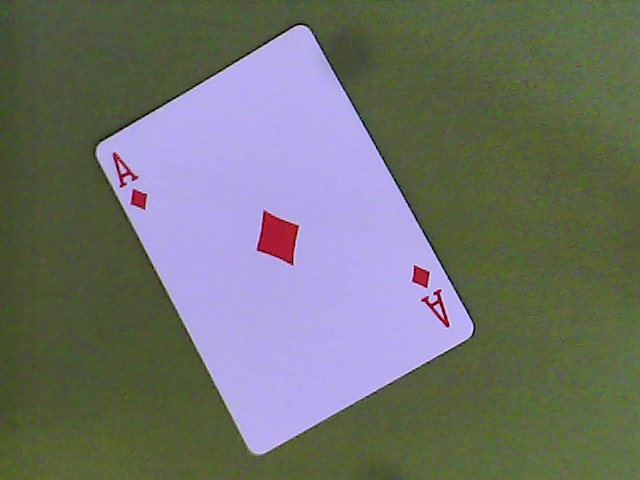
\includegraphics[width=0.06\linewidth]{sve-karte/img2}
		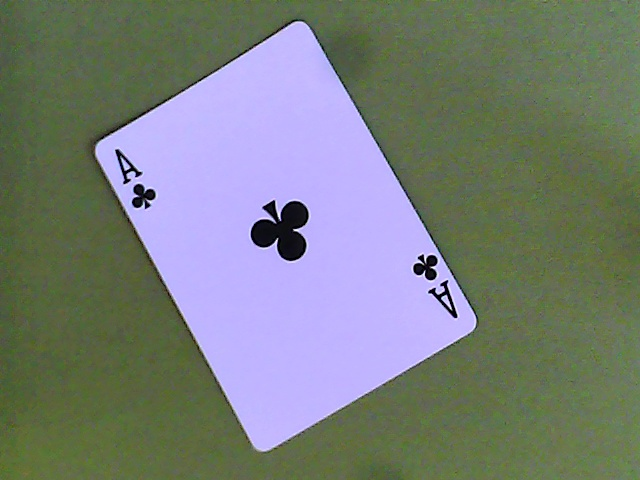
\includegraphics[width=0.06\linewidth]{sve-karte/img3}
		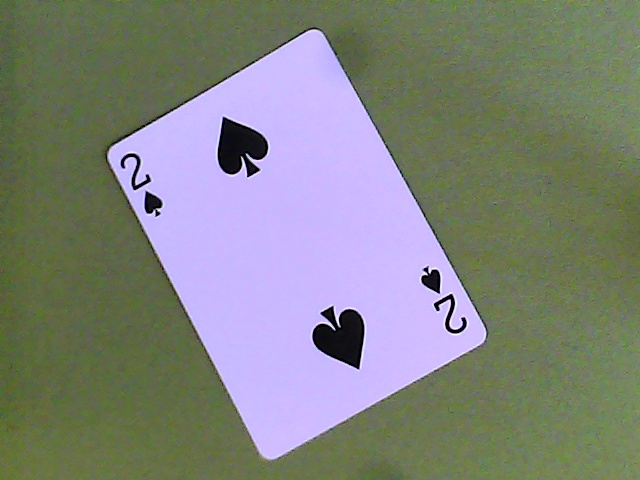
\includegraphics[width=0.06\linewidth]{sve-karte/img4}
		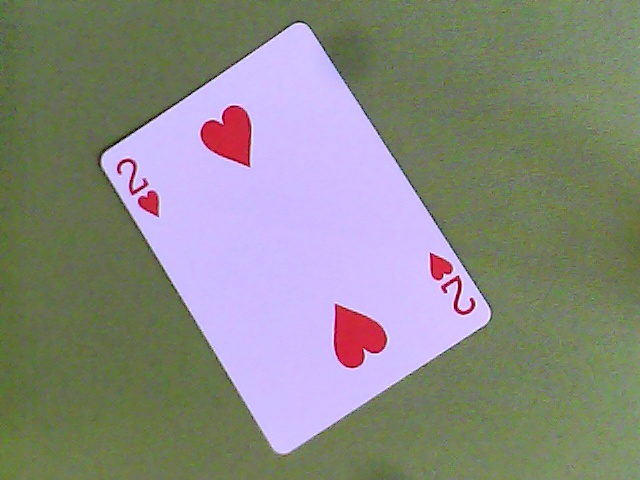
\includegraphics[width=0.06\linewidth]{sve-karte/img5}
		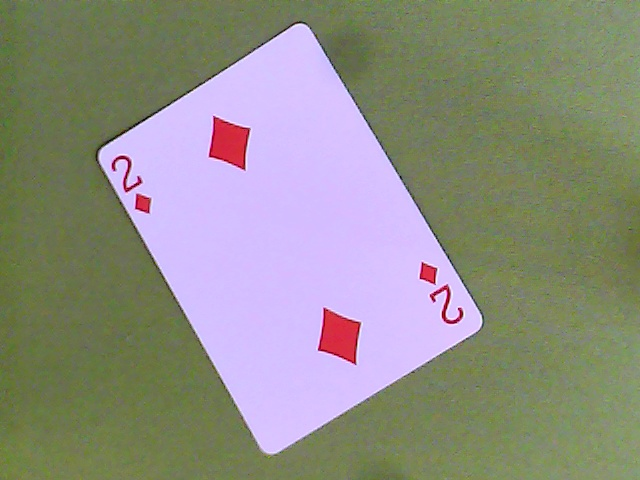
\includegraphics[width=0.06\linewidth]{sve-karte/img6}
		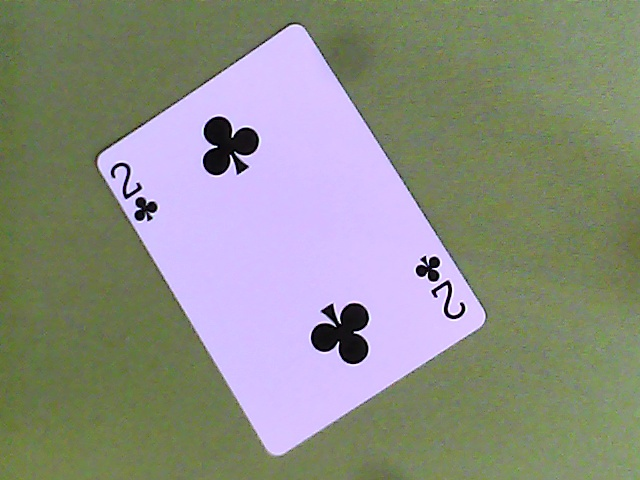
\includegraphics[width=0.06\linewidth]{sve-karte/img7}
		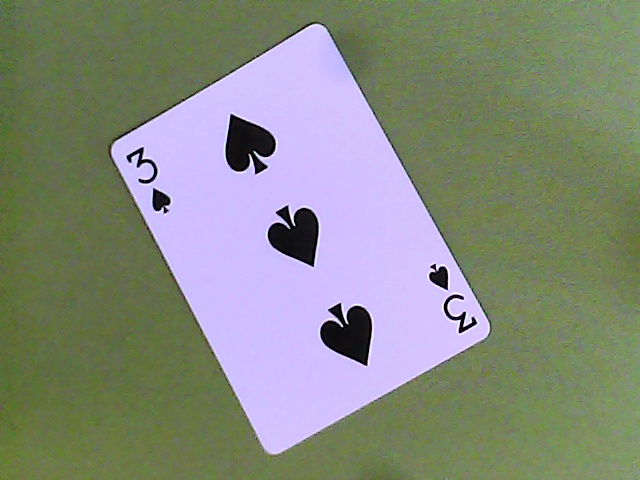
\includegraphics[width=0.06\linewidth]{sve-karte/img8}
		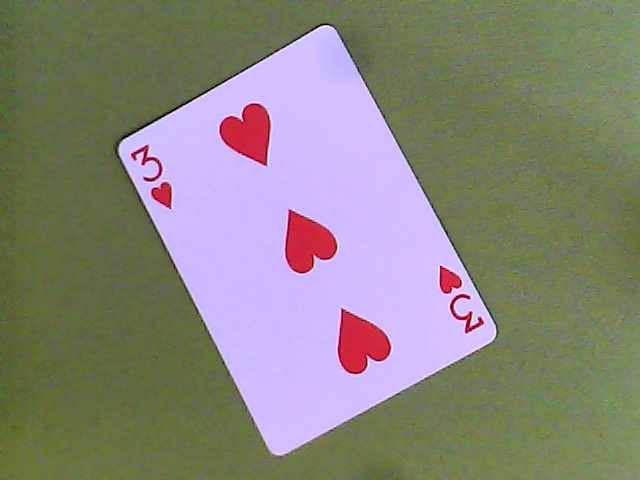
\includegraphics[width=0.06\linewidth]{sve-karte/img9}
		\includegraphics[width=0.06\linewidth]{sve-karte/img10}
		\includegraphics[width=0.06\linewidth]{sve-karte/img11}
		\includegraphics[width=0.06\linewidth]{sve-karte/img12}\\[3px]
		\includegraphics[width=0.06\linewidth]{sve-karte/img13}
		\includegraphics[width=0.06\linewidth]{sve-karte/img14}
		\includegraphics[width=0.06\linewidth]{sve-karte/img15}
		\includegraphics[width=0.06\linewidth]{sve-karte/img16}
		\includegraphics[width=0.06\linewidth]{sve-karte/img17}
		\includegraphics[width=0.06\linewidth]{sve-karte/img18}
		\includegraphics[width=0.06\linewidth]{sve-karte/img19}
		\includegraphics[width=0.06\linewidth]{sve-karte/img20}
		\includegraphics[width=0.06\linewidth]{sve-karte/img21}
		\includegraphics[width=0.06\linewidth]{sve-karte/img22}
		\includegraphics[width=0.06\linewidth]{sve-karte/img23}
		\includegraphics[width=0.06\linewidth]{sve-karte/img24}
		\includegraphics[width=0.06\linewidth]{sve-karte/img25}\\[3px]
		\includegraphics[width=0.06\linewidth]{sve-karte/img26}
		\includegraphics[width=0.06\linewidth]{sve-karte/img27}
		\includegraphics[width=0.06\linewidth]{sve-karte/img28}
		\includegraphics[width=0.06\linewidth]{sve-karte/img29}
		\includegraphics[width=0.06\linewidth]{sve-karte/img30}
		\includegraphics[width=0.06\linewidth]{sve-karte/img31}
		\includegraphics[width=0.06\linewidth]{sve-karte/img32}
		\includegraphics[width=0.06\linewidth]{sve-karte/img33}
		\includegraphics[width=0.06\linewidth]{sve-karte/img34}
		\includegraphics[width=0.06\linewidth]{sve-karte/img35}
		\includegraphics[width=0.06\linewidth]{sve-karte/img36}
		\includegraphics[width=0.06\linewidth]{sve-karte/img37}
		\includegraphics[width=0.06\linewidth]{sve-karte/img38}\\[3px]
		\includegraphics[width=0.06\linewidth]{sve-karte/img39}
		\includegraphics[width=0.06\linewidth]{sve-karte/img40}
		\includegraphics[width=0.06\linewidth]{sve-karte/img41}
		\includegraphics[width=0.06\linewidth]{sve-karte/img42}
		\includegraphics[width=0.06\linewidth]{sve-karte/img43}
		\includegraphics[width=0.06\linewidth]{sve-karte/img44}
		\includegraphics[width=0.06\linewidth]{sve-karte/img45}
		\includegraphics[width=0.06\linewidth]{sve-karte/img46}
		\includegraphics[width=0.06\linewidth]{sve-karte/img47}
		\includegraphics[width=0.06\linewidth]{sve-karte/img48}
		\includegraphics[width=0.06\linewidth]{sve-karte/img49}
		\includegraphics[width=0.06\linewidth]{sve-karte/img50}
		\includegraphics[width=0.06\linewidth]{sve-karte/img51}\\[3px]
		\caption{$52$ testne slike}
		\label{fig:testimages}
\end{figure}

\begin{figure}[H]
\begin{subfigure}{.5\textwidth}
  \centering
  \includegraphics[width=0.8\linewidth]{sve-karte/img0.jpg}
  \caption{Izvorni $A$ pik}
  \label{fig:asource}
\end{subfigure}%
\begin{subfigure}{.5\textwidth}
  \centering
  \includegraphics[width=.5\linewidth]{acesucks.jpg}
  \caption{Neuspjeli pokušaj dilatacije i otvaranja na $A$ pik}
  \label{fig:openedace}
\end{subfigure}
\caption{Problem karte $A$ pik}
\label{fig:aceproblem}
\end{figure}

Ostatak testiranja bi se trebao provesti s kartama u drugim uvjetima, npr. lošije osvjetljenje, različita pozadina, pod različitim kutovima, što bi pokazalo koliko je sustav zapravo efikasan. 

\begin{table}[ht]
\caption{Rezultati testiranja} % title of Table
\centering % used for centering table
\begin{tabular}{c c c c c} % centered columns (4 columns)
\hline\hline %inserts double horizontal lines
$\downarrow$ Jačina / Oznaka boje $\rightarrow$ & \ding{171} & \ding{170} & \ding{169} & \ding{168}\\ [0.5ex] % inserts table
%heading
\hline % inserts single horizontal line
A & \parbox{2cm}{\centering \ding{55}\\ $t$: $2.28s$} & \parbox{2cm}{\centering \checkmark \\ $t$: $2.37s$} & \parbox{2cm}{\centering \checkmark \\ $t$: $2.4s$} & \parbox{2cm}{\centering \checkmark \\ $t$: $2.26s$} \\ [2ex]
\hline
2 & \parbox{2cm}{\centering \checkmark\\ $t$: $2.32s$} & \parbox{2cm}{\centering \checkmark \\ $t$: $2.33s$} & \parbox{2cm}{\centering \checkmark \\ $t$: $2.33s$} & \parbox{2cm}{\centering \checkmark \\ $t$: $2.24s$} \\ [2ex]
\hline
3 & \parbox{2cm}{\centering \checkmark\\ $t$: $2.29s$} & \parbox{2cm}{\centering \checkmark \\ $t$: $2.32s$} & \parbox{2cm}{\centering \checkmark \\ $t$: $2.33s$} & \parbox{2cm}{\centering \checkmark \\ $t$: $2.54s$} \\ [2ex]
\hline
4 & \parbox{2cm}{\centering \checkmark\\ $t$: $2.26s$} & \parbox{2cm}{\centering \checkmark \\ $t$: $2.26s$} & \parbox{2cm}{\centering \checkmark \\ $t$: $2.35s$} & \parbox{2cm}{\centering \checkmark \\ $t$: $2.23s$} \\  [2ex]
\hline
5 & \parbox{2cm}{\centering \checkmark\\ $t$: $2.26s$} & \parbox{2cm}{\centering \checkmark \\ $t$: $2.3s$} & \parbox{2cm}{\centering \checkmark \\ $t$: $2.32s$} & \parbox{2cm}{\centering \checkmark \\ $t$: $2.29s$} \\ [2ex]
\hline
6 & \parbox{2cm}{\centering \checkmark\\ $t$: $2.24s$} & \parbox{2cm}{\centering \checkmark \\ $t$: $2.26s$} & \parbox{2cm}{\centering \checkmark \\ $t$: $2.35s$} & \parbox{2cm}{\centering \checkmark \\ $t$: $2.2s$} \\ [2ex]
\hline
7 & \parbox{2cm}{\centering \checkmark\\ $t$: $2.23s$} & \parbox{2cm}{\centering \checkmark \\ $t$: $2.27s$} & \parbox{2cm}{\centering \checkmark \\ $t$: $2.34s$} & \parbox{2cm}{\centering \checkmark \\ $t$: $2.22s$} \\ [2ex]
\hline
8 & \parbox{2cm}{\centering \checkmark\\ $t$: $2.26s$} & \parbox{2cm}{\centering \checkmark \\ $t$: $2.22s$} & \parbox{2cm}{\centering \checkmark \\ $t$: $2.24s$} & \parbox{2cm}{\centering \checkmark \\ $t$: $2.2s$} \\ [2ex]
\hline
9 & \parbox{2cm}{\centering \checkmark\\ $t$: $2.2s$} & \parbox{2cm}{\centering \checkmark \\ $t$: $2.2s$} & \parbox{2cm}{\centering \checkmark \\ $t$: $2.31s$} & \parbox{2cm}{\centering \checkmark \\ $t$: $2.12s$} \\ [2ex]
\hline
10 & \parbox{2cm}{\centering \checkmark\\ $t$: $2.17s$} & \parbox{2cm}{\centering \checkmark \\ $t$: $2.27s$} & \parbox{2cm}{\centering \checkmark \\ $t$: $2.25s$} & \parbox{2cm}{\centering \checkmark \\ $t$: $2.11s$} \\ [2ex]
\hline
J & \parbox{2cm}{\centering \checkmark\\ $t$: $2.3s$} & \parbox{2cm}{\centering \checkmark \\ $t$: $2.29s$} & \parbox{2cm}{\centering \checkmark \\ $t$: $2.38s$} & \parbox{2cm}{\centering \checkmark \\ $t$: $2.24s$} \\ [2ex]
\hline
Q & \parbox{2cm}{\centering \checkmark\\ $t$: $2.34s$} & \parbox{2cm}{\centering \checkmark \\ $t$: $2.37s$} & \parbox{2cm}{\centering \checkmark \\ $t$: $2.4s$} & \parbox{2cm}{\centering \checkmark \\ $t$: $2.46s$} \\ [2ex]
\hline
K & \parbox{2cm}{\centering \checkmark\\ $t$: $2.71s$} & \parbox{2cm}{\centering \checkmark \\ $t$: $2.38s$} & \parbox{2cm}{\centering \checkmark \\ $t$: $2.41s$} & \parbox{2cm}{\centering \checkmark \\ $t$: $2.82s$} \\ [2ex]
\hline %inserts single line
\end{tabular}
\label{table:stats} % is used to refer this table in the text
\end{table}

\chapter{Zaključak}
\label{chap:concl}
\hspace*{0.5cm}Tijekom izrade rada mnogo novih stvari je naučeno iz područja obrade slike i računalnog vida, a posebno iz dijela matematičke morfologije, ali i ostalih tehnika obrade slike poput detekcije rubova, pronalaženja kontura, primjenjivanja pragova na slike, itd. \\
\hspace*{0.5cm}Rezultati dobiveni ovom metodom su dobri ukoliko raspolažemo slikama koje su dobro osvijetljene, ali se ne bi trebalo tu zaustaviti. Sljedeći korak bi trebao biti popravljanje sustava kako bi davao ispravne rezultate za različite uvjete. Ukoliko bi bilo lošije osvjetljenje, trebao bi se koristiti prilagodljivi prag (engl. \textit{adaptive threshold}) koji ne bi uzimao jednu vrijednost i prema njoj mijenjao sliku, nego bi za svaki blok slike (veličina bloka se zadaje prilikom pozivanja funkcije) računao prag te bi na posljetku slika bila dovoljno izoštrena kako bi se mogle prepoznati konture te vršiti daljnji proces klasifikacije. Također, vremenski rezultati bi se mogli popraviti koristeći \code{C++}, ali vjerojatno najbolje rješenje bi bila neuronska mreža zbog brzine klasificiranja. \\
\hspace*{0.5cm}Krajnji cilj je spojiti ovaj sustav s robotskom rukom koja bi mogla prepoznavati karte preko kamere te bi bilo moguće igrati neke kartaške igre protiv robota što bi bilo zanimljivo te napraviti grafičko sučelje za lakše snalaženje i preglednije ispise tijekom procesa prepoznavanja karata. 
\bibliography{literatura}
\bibliographystyle{unsrt}


\begin{sazetak}
Ovaj rad razmatra prepoznavanje igraćih karata korištenjem tehnika obrade slike. Obrada slika obavlja se kroz niz koraka: pronalaženje rubova, pronalaženje najbolje četverokutne konture, perspektivna transformacija. Prepoznavanje se također vrši preko obrade slike korištenjem algoritama \textit{Floodfill} (za brojeve) te pogodi i promaši transformacijom (za slova i oznaku boje). Postupak se pokazao djelomičnom uspješnim. Dobiveni su točni rezultati na $51$ od $52$ testne slike pri dobrom osvjetljenju, dok za lošije osvjetljenje su i malo lošiji rezultati. Sve metode i postupci korišteni pri prepoznavanju igraćih karata detaljno su opisani kroz rad.

\kljucnerijeci{prepoznavanje igraćih karata, pronalaženje kontura, detekcija rubova, matematička morfologija, floodfill, pogodi i promaši transformacija, perspektivna transformacija.}
\end{sazetak}

% TODO: Navedite naslov na engleskom jeziku.
\engtitle{Playing card recognition system}
\begin{abstract}
This thesis presents implementation of playing cards recognition system using image processing. Processing is done through several steps: edge detection, finding quadrilateral contour, perspective transform. Recognition is also done by using image processing algorithms such as \textit{Floodfill} (number detection) and Hit-and-miss transform (for letters and suits). The procedure proved to be partially successful. $51$ out of $52$ test cards are classified correctly in well-lit environment, while the results in low-lit environment are slightly worse. All methods and procedures used in playing card recognition are described in detail in thesis.

\keywords{playing cards recognition, contour finding, edge detection, mathematical morphology, floodfill, hit-and-miss transfrom, perspective transform.}
\end{abstract}

\end{document}
